% Basic LaTeX template for NE 204 lab report
\documentclass[11pt]{article}

%==============================================================================
%%% Everything between the "="'s is the preamble.
%%% Define packages and meta data here

% Common packages
\usepackage{amsmath}    % Expanded math
\usepackage{amssymb}    % Expanded math symbols
\usepackage{graphicx}   % For images
\usepackage{float}
\usepackage{subcaption} % To use images together
\usepackage{pgfplotstable} % To make tables
\usepackage{array} % To make tables


% All images/figures will be stored in the images folder.
% Specify that here so pdflatex knows where to look for images.
\graphicspath{{./images/}}

% Metadata
\title{Lab 0: HPGe Spectroscopic Calibration}
\author{Grey Batie}
\date{\today}
%==============================================================================

\begin{document}

% Compile metadata from preamble into a nicely-rendered title section
\maketitle

% The *'s next so section/subsection definitions suppresses numbering
\section*{Introduction}
\label{sec:intro}

Gamma rays are quantized electromagnetic radiation produced
by nuclear transitions. These uncharged particles cannot directly ionize or
excite atoms in material it traverses through, making them difficult to be
detected directly. Therefore, it is necessary that some fraction of the incident
photon's energy to be transferred to an electron in the absorbing
material. These fast electrons can then induce excitations or ionization which
 provide valuable information about the nature of the incident gamma rays.

The sensitive volume of a radiation detector serves as a
gamma-ray spectrometer, measuring the intensity and energy of incident gamma rays.
It is advantageous for this region to be composed of solid material, to increase
the probability of a photon interacting inside of it. High purity germanium detectors,
a common type of semi-conductor detector, employ a highly absorptive germanium crystal,
 in addition to being compact, and offering
fast timing characteristics \cite{knoll}.

These devices must be calibrated so that the signal produced
corresponds to the correct incident radiation energy. Most calibration
procedures involve using a known gamma ray source to assign the output
voltage of the detector with the corresponding known gamma ray energy. Once
a detector is properly calibrated it is capable of measuring unknown sources
to better understand a radiation field of interest.


\section*{Methods}
\label{sec:meth}
In this lab, raw (uncalibrated) data was collected from five different
radiation sources:  $^{241}$Am, $^{133}$Ba, $^{60}$Co, $^{137}$Cs, and $^{152}$Eu.
The measurements were performed using a coaxial HPGe detector and a 13-bit resolution MCA,
yielding 8192-bin spectra. It is assumed that each of these measurements were
taken with each source at the same location and distance from the detector.
All raw data collected is plotted in Figure ~\ref{fig:raw}.



\begin{figure}[H]
\begin{center}
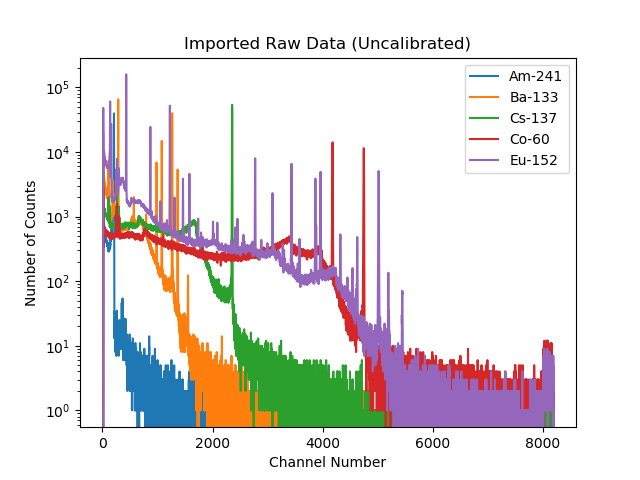
\includegraphics[width=.7\linewidth]{../images/rawdata.png}
\caption{Calibrated Americium and Cesium Spectrum \label{fig:raw}}
\end{center}

\end{figure}


The gamma energies of interest are given in Table
\ref{tab:src}, were primarily chosen based on their
branching ratios, as those with the highest branching ratios tend to be
the most visible within a spectrum.

\begin{table}[H]
  \begin{center}
    \begin{tabular}{l|r}
      \textbf{Source} & \textbf{Energy (keV)}\\
      \hline
      $^{241}$Am    &  59.541    \\
      $^{133}$Ba    &  80.997    \\
                    &  356.017   \\
      $^{60}$Co     &  1173.237  \\
                    &  1332.501  \\
      $^{137}$Cs    &  661.657   \\
      $^{152}$Eu    &  121.781   \\
                    &  1408.006  \\
    \end{tabular}
    \caption{Gamma-ray lines used in the calibration}
    \label{tab:src}
  \end{center}
\end{table}

A simple linear calibration method can be employed two different energy
peaks and the channels in the raw data where these peaks are believed to
correspond to.


\begin{equation}
m=\frac{E_2-E_1}{chan_2-chan_1}
\end{equation}

where m is the slope of the linear regression line, and  $E_1$ and
$chan_1$ are a single gamma energy and corresponding channel number.

The general equation of the linear regression line is:

\begin{equation}
Energy-E_1=m(channel-chan_1)
\end{equation}


\section*{Results}
\label{sec:res}

The equation of the linear regression line for this data using the 59.541 keV
peak of $^{241}$Am and the  661.657 keV peak from $^{137}$Cs.

\begin{equation}
Energy=0.280576(channel)+1.181092
\end{equation}

This model is then used to calibrate both $^{241}$Am and $^{137}$Cs
data, and is displayed in Figure \ref{fig:fit}.



\begin{figure}[H]
\begin{center}
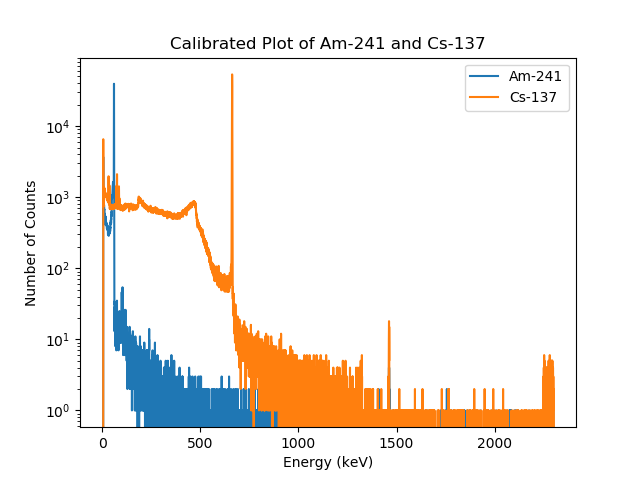
\includegraphics[width=.7\linewidth]{cal_AmCs.png}
\caption{Calibrated Americium and Cesium Spectrum \label{fig:fit}}
\end{center}

\end{figure}



Comparing the calibrated pulse height spectrum of $^{133}$Ba
to its true values as specified in the nuclear data literature
we find that the model is sufficiently accurate. The full comparison is
displayed in the table below.

\pgfplotstabletypeset[%
   fixed zerofill,
   precision=4,
   col sep=space,
   dec sep align,
   columns/0/.style ={column name=Actual Energy (KeV)},
   columns/1/.style ={column name=Calibrated Energy (KeV)},
   columns/2/.style ={column name=Percent Difference (\%)},
]{./images/peakdiffquant.csv}


\section*{Discussion}
\label{sec:disc}
Calibrating a gamma ray spectrum is vital for observing
and measuring any gamma radiation field. From the data
provided, a simple linear fit between 59.541 keV and 661.657 keV
has shown to be sufficiently accurate.

For future work and improvement upon this energy calibration, more than
two peaks could have been used to determine the parameters of linear
calibration, or a higher order polynomial regression method.


% Bibliography
\bibliographystyle{plain}
% Refers to a bibtex file in the current dir named "references.bib"
\bibliography{references}

\end{document}
